\documentclass{article}
\usepackage[left=0.85in,top=0.6in,right=0.85in]{geometry}
\usepackage{booktabs}
\usepackage{array,multirow}
\usepackage{graphicx}
\usepackage{pifont}
\usepackage{amssymb}
\usepackage{enumitem}
\usepackage{floatflt}
\usepackage{hyperref}
\usepackage[table]{xcolor}

\title{\Huge Cherry Dropper}
\author{\huge Group 26}
\begin{document}
\maketitle
\begin{center}
\setlength{\arrayrulewidth}{1mm}
\setlength{\tabcolsep}{18pt}
\renewcommand{\arraystretch}{2.5}
 
{\rowcolors{3}{green!80!yellow!50}{green!70!yellow!40}
\begin{tabular}{ |p{3cm}|p{3cm}|  }
\hline
\multicolumn{2}{|c|}{\huge Optimus} \\
\hline
 ROLL NO.  & NAME\\
\hline
 140050029 & B.Avinash \\
 140050069   & Suraj Geddam \\
 140050087 & Ashna Gaur \\
\hline
\end{tabular}
}
\\[5\baselineskip]
{\huge CS251 Project- Box 2D}
\\[2\baselineskip]
Prepared for Software Systems lab: \\[1\baselineskip]
{\large Instructor} : \textbf{Prof. Sharat Chandran }\\[1\baselineskip]
Autumn 2015 \\
\end{center}

\newpage
\section*{\huge Table of Contents:} \label{Contents}
\begin{enumerate}
    \LARGE  \item Introduction
    \begin{enumerate} [label*=\arabic*.]
        \large \item Project Design
        \large \item Description
    \end{enumerate}
    \LARGE  \item Objects of the Project
    \begin{enumerate} [label*=\arabic*.]
        \large \item Pendulum
        \large \item Dominos
        \large \item Gears
        \large \item Train of small spheres
        \large \item Hydraulic lift
        \large \item Revolving plank
        \large \item Another Dominos
        \large \item Fluid in the box
        \large \item The boat 
        \large \item Pulley joint
        \large \item Cake 
    \end{enumerate}
    \LARGE  \item Software Applications Implemented
    \begin{enumerate} [label*=\arabic*.]
        \large \item Documentation
        \large \item Profiling
        \large \item Webpage Preparation
        \large \item Makefiles
    \end{enumerate}
    \LARGE  \item Work Distribution
    \begin{enumerate} [label*=\arabic*.]
        \large \item B.Avinash
        \large \item Suraj Geddam
        \large \item Ashna Gaur
        \large \item Honour Code
    \end{enumerate}
    \LARGE  \item Difficulties and Deviations
    \begin{enumerate} [label*=\arabic*.]
        \large \item Difficulties Faced And how we overcame them
        \large \item What we didn't implement
    \end{enumerate}
\end{enumerate}
 
%\begin{figure}[h]
%\centering
%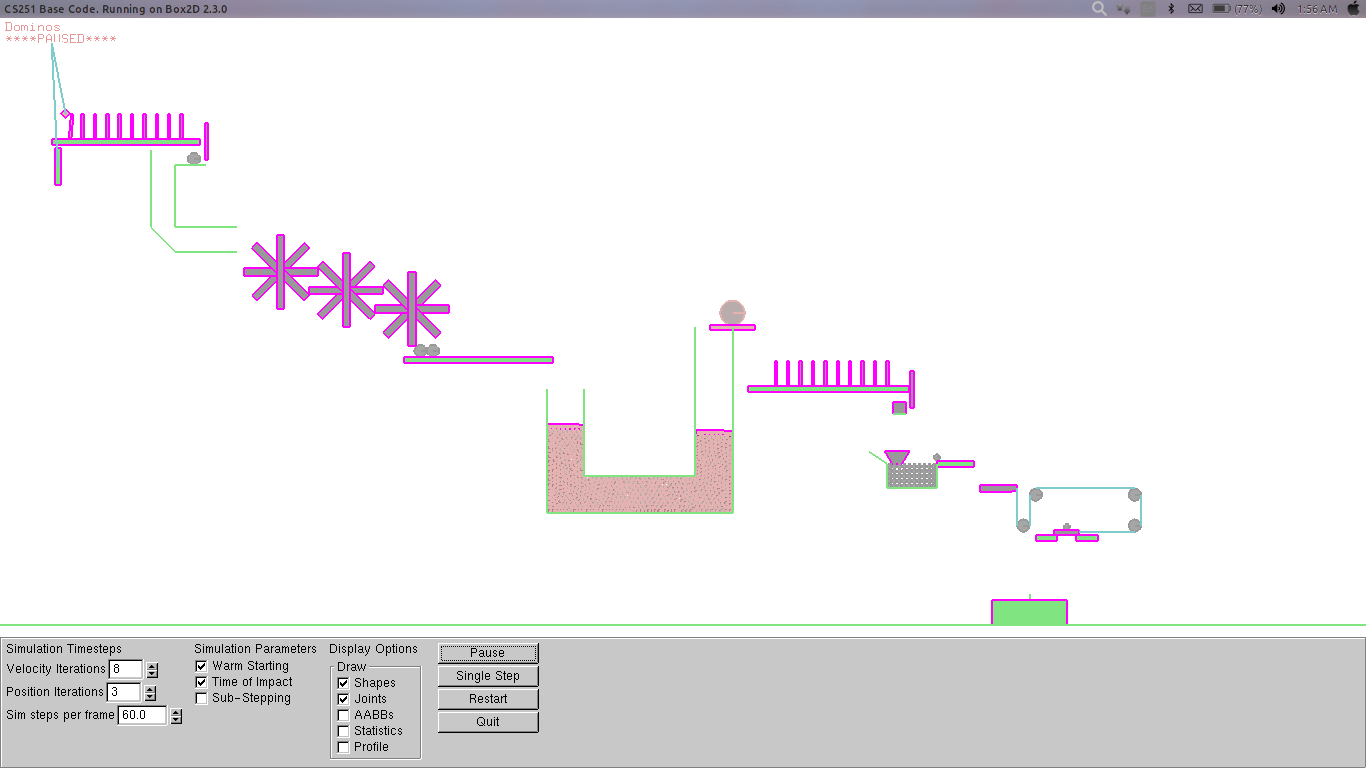
\includegraphics[width=1 \linewidth]{suraj.png}
%\caption{\large Our Box2D Design}
%\end{figure}
\begin{itemize}
	\item[] \textbf{\LARGE Project Design} \vspace{0cm} \\
	\large This project idea is a simulation which is based on placing a cherry on the cake.We were inspired from many daily-life simulations and by the one given in the Lab03 .  \vspace{0.2cm}
	\item[] \textbf{\LARGE Description} \vspace{0cm} \\
	\large In this simulation, the bob of the left most pendulum hits the first domino which in return hit one by one and finally the revolving domino hits the small ball which goes and turns the 3 gears and in turn initiates a train of small balls to go and fall on a hydraulic lift  which makes the heavy ball on the plank on the right top of the lift. The heavy ball initiates the dominos to go and hit the small box.\\
 \end{itemize}

\begin{itemize}
 \item[] \textbf{\LARGE Objects of the Project} \\
        \begin{itemize}[label=$\blacksquare$] \vspace{0cm}
            \item \textbf{\Large Pendulum} 
        \end{itemize}
        \large Pendulum at the top left corner in the below image is the start of the simulation. The bob hits the first domino. \\ \vspace{0.2cm}

        \begin{itemize}[label=$\blacksquare$] \vspace{0cm}
            \item \textbf{\Large Dominos } 
        \end{itemize} 
        \large The first domino which in return hit one by one and finally the revolving domino hits the small ball which goes to the gears. \\ \vspace{0.2 cm}

        \begin{itemize}[label=$\blacksquare$] \vspace{0cm}
            \item \textbf{\Large Gears } 
        \end{itemize}
        \large The small ball rotates the first gear anti-clockwise which rotates the second gear in clockwise and thus the third gear rotates in anti-clockwise direction and hits the train of small spheres .\\ \vspace{0.55 cm}

        \begin{itemize}[label=$\blacksquare$] \vspace{0cm}
            \item \textbf{\Large Train of small spheres } 
        \end{itemize}
        \large The train of these spheres follow the same as the dominos above and fall on one side of the Hydraulic lift.\\ \vspace{0.2 cm}

        \begin{itemize}[label=$\blacksquare$] \vspace{0cm}
            \item \textbf{\Large Hydraulic lift } 
        \end{itemize}
        \large The name itself indicates the function.The balls on one side of the lift cause the rise of height to the other side due to which the plank hits the revolving plank. \\ \vspace{0.2 cm}

        \begin{itemize}[label=$\blacksquare$] \vspace{0cm}
            \item \textbf{\Large Revolving plank } 
        \end{itemize}
        \large The revolving plank is set on the right most end of the Hydraulic lift and a heavy sphere is placed on the plank.\\ \vspace{0.2 cm}
\newpage
        \begin{itemize}[label=$\blacksquare$] \vspace{0cm}
            \item \textbf{\Large Another Dominos } 
        \end{itemize}
        \large The heavy sphere on the plank falls on the dominos and intiates them to hit the small box placed to the left of revolving domino.\\ \vspace{0.2 cm}

        \begin{itemize}[label=$\blacksquare$] \vspace{0cm}
            \item \textbf{\Large Fluid in the box } 
        \end{itemize}
        \large The fluid in the box is created using samll balls which together act like fluid.\\ \vspace{0.65 cm}

        \begin{itemize}[label=$\blacksquare$] \vspace{0cm}
            \item \textbf{\Large the boat} 
        \end{itemize}
        \large Th boat is constructed using a polygon with 4 vertices and is plced on the top of the fluid which on getting hit by the box flows to the other end and hits the small ball in return. \\ \vspace{0.65 cm}

        \begin{itemize}[label=$\blacksquare$] \vspace{0cm}
            \item \textbf{\Large Pulley Joint} 
        \end{itemize}
        \large The small ball falls on the pulley joint and disturbs the cherry which rests on the plank.\\ \vspace{0.65 cm}
        
        \begin{itemize}[label=$\blacksquare$] \vspace{0cm}
            \item \textbf{\Large Cake} 
        \end{itemize}
        \large Cake is made by polygon of 4 vertices and the cherry comes from the pulley joint settles on the cake and hence the simulation is complete.\\ \vspace{0.65 cm}
    \end{itemize}

\begin{itemize}
	\item[] \textbf{\LARGE Software Applications Implemented} \\
        \begin{itemize}[label=$\blacksquare$] \vspace{0cm}

            \item \textbf{\Large Documentation }\\
            \large We used doxygen to document our project.We have written meaningful comments in order to increase the understandability of other programmers who try to understand our project. We can get the documentation by writing "make doc" in the project direcory(on the terminal). \vspace{0.20 cm}

            \item \textbf{\Large Profiling}\\ 
            \large The code profile can be generated by the command "make profile" in the project directory . \vspace{0.20 cm}

            \item \textbf{\Large Webpage Preparation}\\ 
            \large We created a webpage for the project which is available at {\large {\bf HOMEPAGE:} \ \url{www.cse.iitb.ac.in/~avinash}}. \vspace{0.20 cm}

            \item \textbf{\Large Makefile}\\ 
            \large We created a makefile which can be used to cmpile all the files, do the profiling, create the executables, create the documentation of the project ,report of the project and clean all the unneccessary files. \vspace{0.2 cm}


 \end{itemize}
        \end{itemize}


\begin{itemize}
	\item[] \textbf{\LARGE Work Distribution} \\
	   \begin{itemize}[label=$\blacksquare$] \vspace{0cm}
           \item \textbf{\Large B.Avinash }\\
           \large Roll Number: 140050029\\ Contribution: 100\% \\ The project was divided into 3 parts which was assigned to the 3 members of the group. Avinash did the first part i.e, the part involving gears and documented his part. He also prepared the report for the project and made the profiling. \vspace{0.2 cm}
           \item \textbf{\Large Suraj Geddam }\\ 
           \large Roll Number: 140050069\\ Contribution: 100\% \\ Suraj did the third and final part of the project which invloves the fluid part and documented his part. He also created the makefile.\vspace{0.2 cm}
           \item \textbf{\Large Ashna Gaur }\\ 
           \large Roll Number: 140050087\\ Contribution: 100\% \\  Ashna did the second part of the project which involved hydraulic lift and documented her completely. She also created the project webpage. \vspace{0.2 cm}
       \end{itemize}
       \item[] \textbf{\LARGE Honour Code} \\ 
       \large We pledge on our honour that we have not given or received any unauthorized assistance on this assignment or any previous task.\\\vspace{0.2 cm}  

	\item[] \textbf{\LARGE Difficulties and Deviations} \\
	\item[] \textbf{\Large Difficulties Faced And how we overcame them} \\
    \large The parts where we faced the main difficulties were to create gears , hydraulic lift and fluid. We tried to understand the code in the gers.h file present in testbed and completed the gears part. And we used small balls in the hydraulic lift instead of fluid which worked fine for us and even looked good.\\ \vspace{0.2 cm}

    \item[] \textbf{\Large What we didn't implement} \\ 
Our intial design was the picture below.
%\begin{figure}[h]
%\centering
%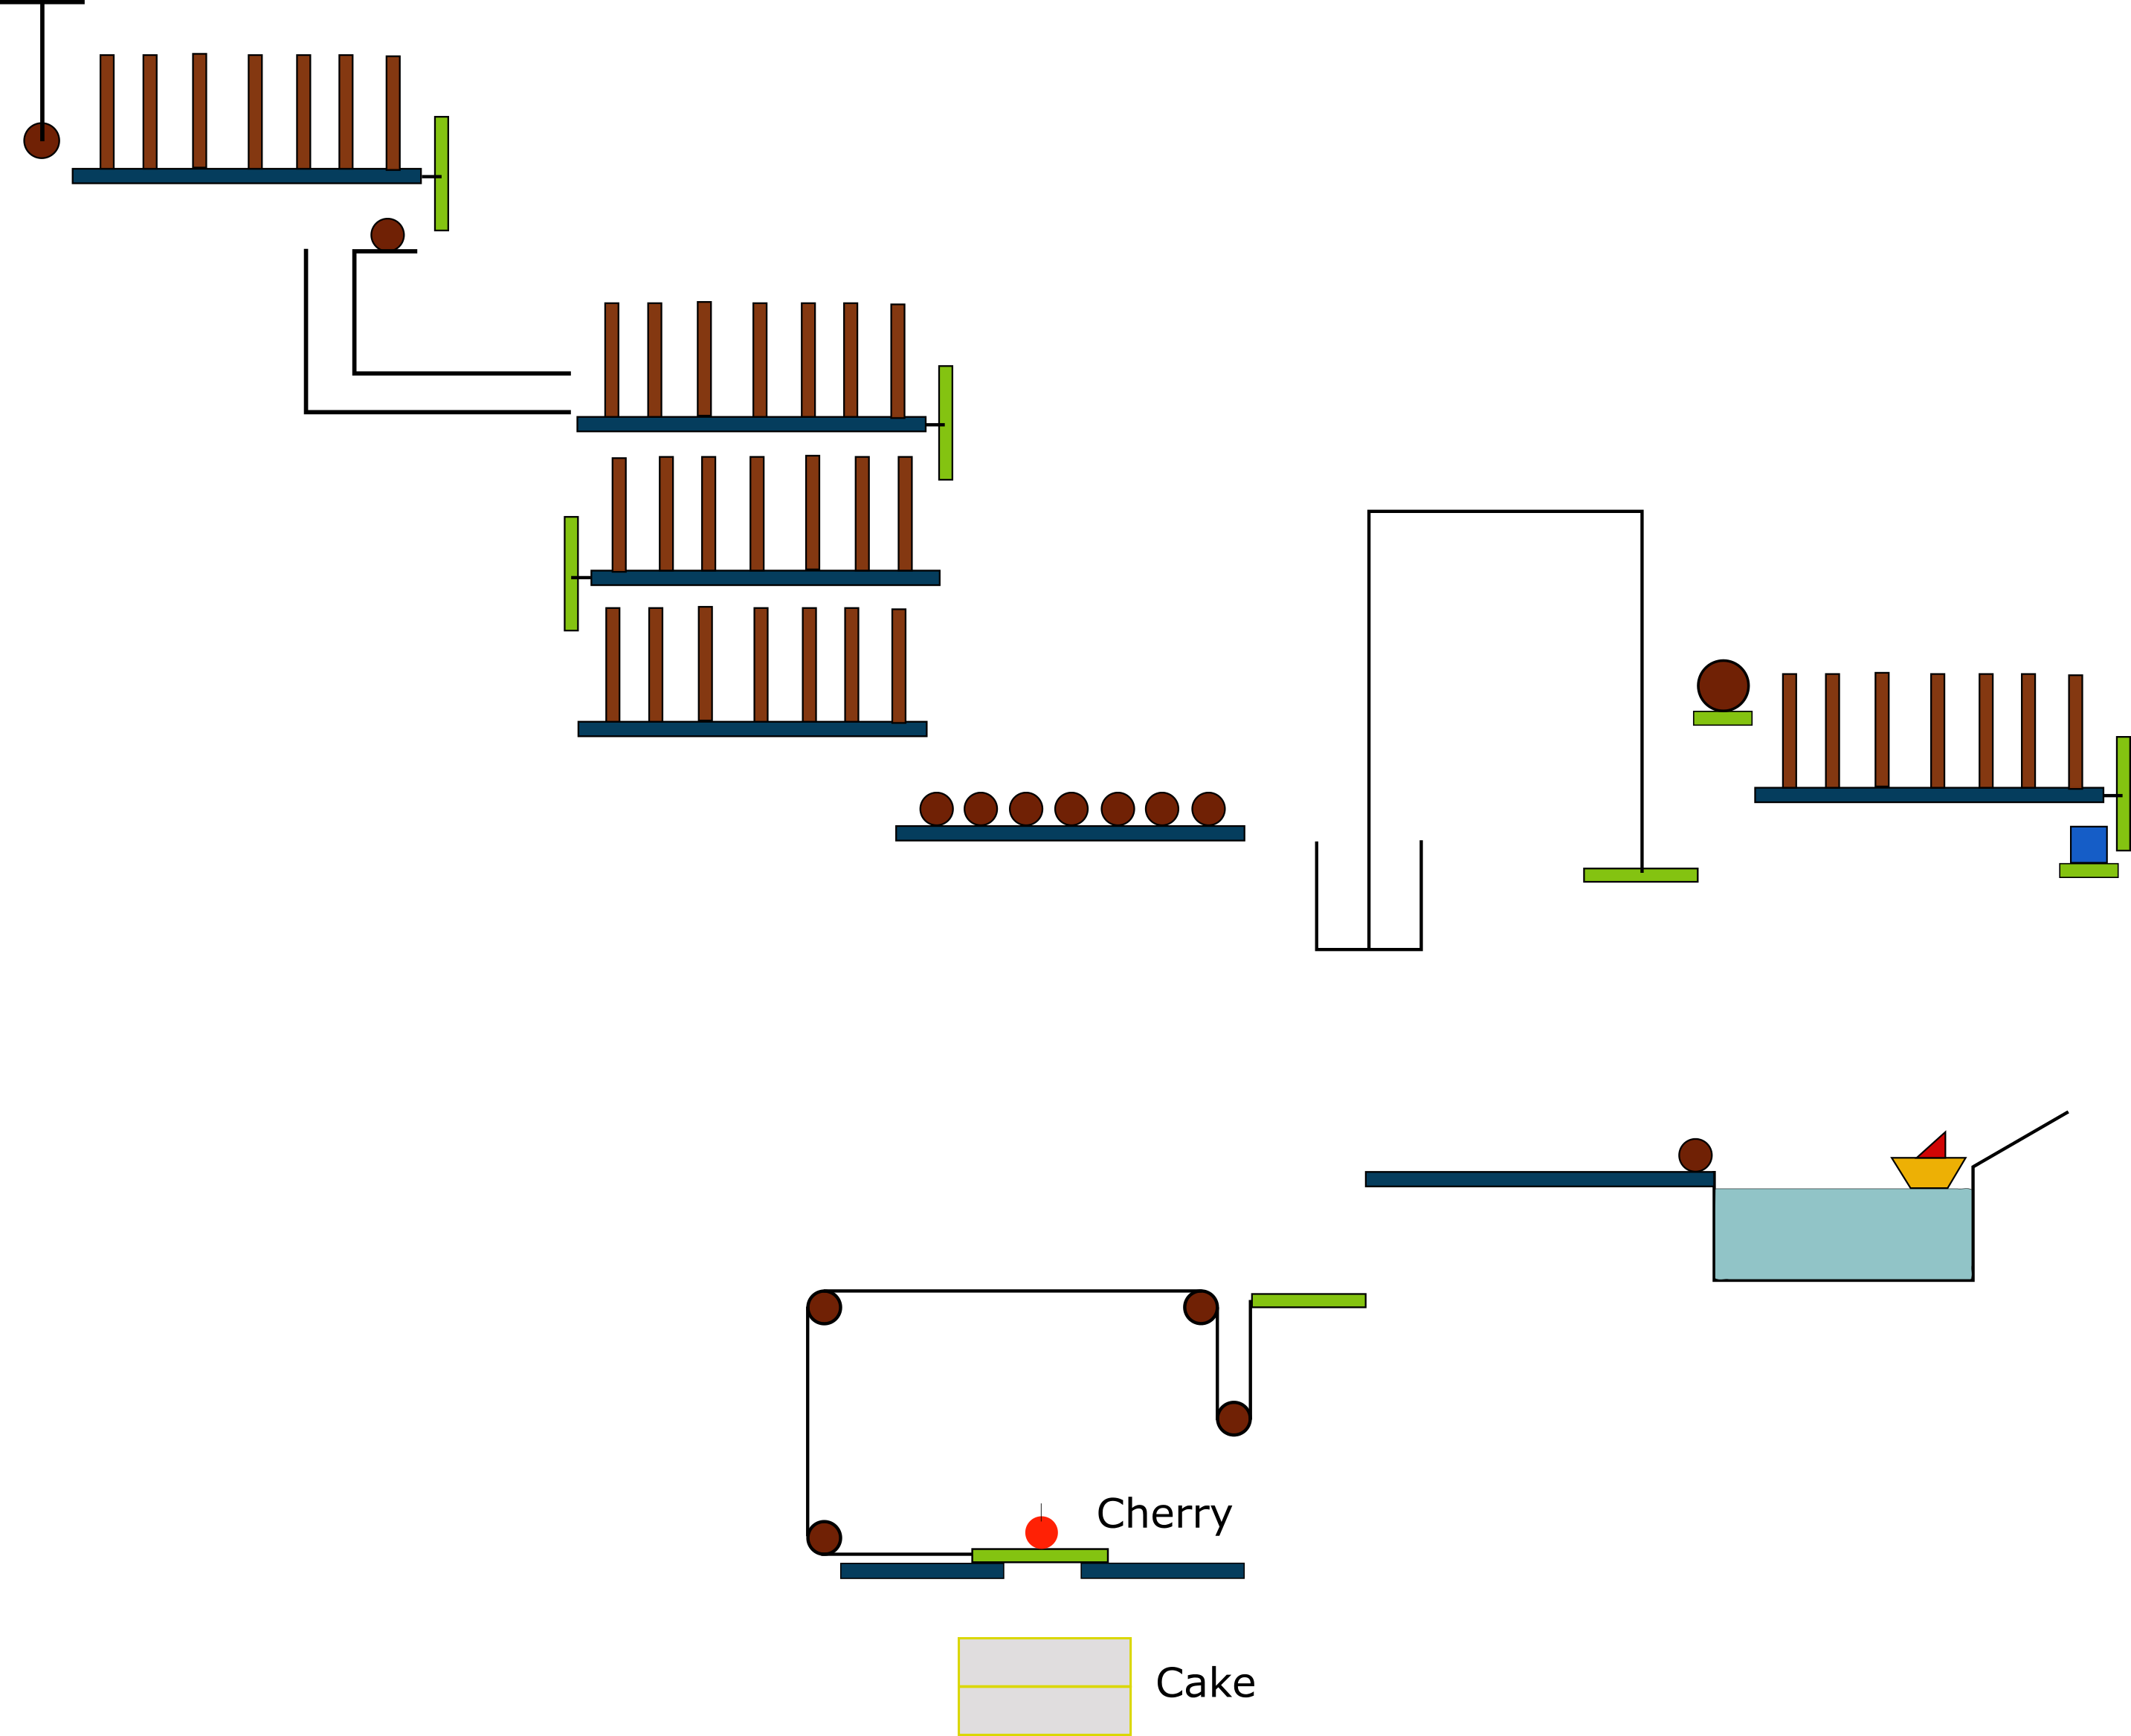
\includegraphics[width=1 \linewidth]{box2D.png}
%\caption{\large Our Box2D Design}
%\end{figure}
But the TA gave us the suggestion to implement gears and simulation of gaseos particles to make it a bit cool. Because this design was pretty similar to the base code and was looking pretty easy. So, we increased the complexity in the design to achieve what we did now.
\\ \vspace{0.2 cm}

\end{itemize}

\end{document}

